\cleardoublepage

\chapter[Introduction]{General Introduction}
\label{ch:introduction}
\thispagestyle{empty}

%\section{}
The importance of communication is apparent from the consequences of it breaking down. Two psychological conditions in which communication is often challenging are social anxiety and autism spectrum conditions. Social anxiety is characterized by fear and anxiety of negative judgement in social situations, and autism spectrum conditions by reduced reciprocating or initiating interactions, reduced use and integration of non-verbal communication, and reduced contextually appropriate communication \citep{apa2013}. Our understanding of the neural mechanisms underlying communication breakdowns in these conditions, however, is limited.

In this thesis, I will focus on finding out whether distinctive neural mechanisms are at the root of the communication problems of these two conditions, from two different angles. Firstly, I will explore whether representing the mental state of others and observing social interactions elicits different neural dynamics in autistic and neurotypical individuals. In addition, the same issue will be investigated for socially anxious and neurotypical individuals, along with the question whether existing differences can be related to state anxiety during social interactions. Secondly, I will examine structure building during language comprehension, such as understanding the structure and meaning of a sentence, in autistic and neurotypical participants, and assess whether this process is supported by differential neural signatures. The verbal and non-verbal research approaches used in this thesis will allow us to more specifically identify the source of communicative difficulties in autism and social anxiety. 

\section{What is needed for successful communication?}

To maintain a successful conversation, many diverse abilities need to be mastered during early life. Speakers need to be able to form thoughts into sounds or letters, words, sentences and finally into a coherent message. The other way around, listeners dissect an array of sounds or letters back into words, sentences and the idea behind the message sent. Learning these structural aspects of language takes place in the first few years of life, in which interaction with parents and caregivers is essential. 

In parallel with learning structural language, we learn to understand that the people around us have goals and intentions and act along them \citep{gergely2002,tomasello2003}. Later in development, around the age of four, we develop the ability to recognize that other people can have a different perspective from our own \citep{wimmer1983}. Generally, the ability to represent the thoughts and beliefs of others is known as mentalizing \citep{premack1978}, and is essential in order to have a successful conversation. When this skill is mastered, children are able to distinguish between their own beliefs and those of other people. Mentalizing might not be necessary to understand simple, clear sentences like "Can you pass me the salt?" at a dinner table. However, everyday language is filled with phrases and utterances of which the literal sense diverges from what the speaker actually means. Someone might say "It's getting cold in here", with the intention to get the listener to shut an open window \citep{vanackeren2012}. Being able to decode the desires, beliefs, and intentions of others is necessary to understand these messages.

With well-developed structural language abilities and mentalizing under one's belt, one can understand a sentence or a story and interpret it in the light of the speaker's background, experiences, and personality. Nevertheless, communication is a dynamic process that involves fine-tuned coordination from the relevant parties. Other abilities are therefore needed to be able to fully understand the message someone is trying to communicate. Examples of these additional abilities are the on-the-fly creation and integration of new words, responding in a timely manner, and integrating the context of a message into its meaning, such as visual information, co-speech gestures, and cultural norms. This compound communication system allows us to understand each other as well and quickly as possible \citep{levinson2020,levinson2024}.
 
\section{What are the neural mechanisms that support these abilities?}

\subsection{Tools}

To understand the inner workings of the human communication system, neuroscientists have been studying the brain in relation to behavior since the latter half of the 19th century. Still, only since the 1980s, a clear picture started to form about the relation between brain function and behavior, due to the inception of cognitive science and the development of neuroimaging tools. Two of the most widely used methods of measuring brain activity are functional magnetic resonance imaging (fMRI) and electroencephalography (EEG). fMRI relies on the assumption that the need for metabolic resources, such as oxygen, increases with regional neuronal activity. Blood flow to these active brain regions will then increase, which can be measured because of the property of oxygen to bind to hemoglobin. Oxygen-poor and oxygen-rich blood have different magnetic properties and therefore allow regional resource consumption to be measured with MRI techniques. The measured signal is known as the BOLD (blood-oxygen level dependent) signal and peaks around 6 seconds following an event. The slowness of this response means that the temporal precision of neural events cannot be assessed precisely. The location of the active brain region, however, can be measured very precisely with fMRI, allowing the detection of regions on a millimeter scale. 

EEG measures brain activity based on different mechanics, namely the summation of electrical currents generated by neurons, specifically the post-synaptic potentials. This summed electrical activity is measured with electrodes at the scalp. Afterwards, it can be analyzed for its changes in voltage following a specific event or stimulus (ERP) or for the rhythms of its synchronized firing patterns (oscillations). In contrast to fMRI, EEG has a poor spatial resolution but a very high temporal resolution. Neural activity can be recorded from mere milliseconds after the occurrence of the event. Even though it is valuable to understand the spatial and temporal properties of brain functions, the field of cognitive neuroscience has a stark tendency to focus on where certain processes are active in the brain instead of when they are active \citep{poeppel2012}. Well-designed EEG experiments are therefore crucial to create informative models on the neural underpinnings of language and communication processing.  
\begin{figure}[!ht]
	\centering
	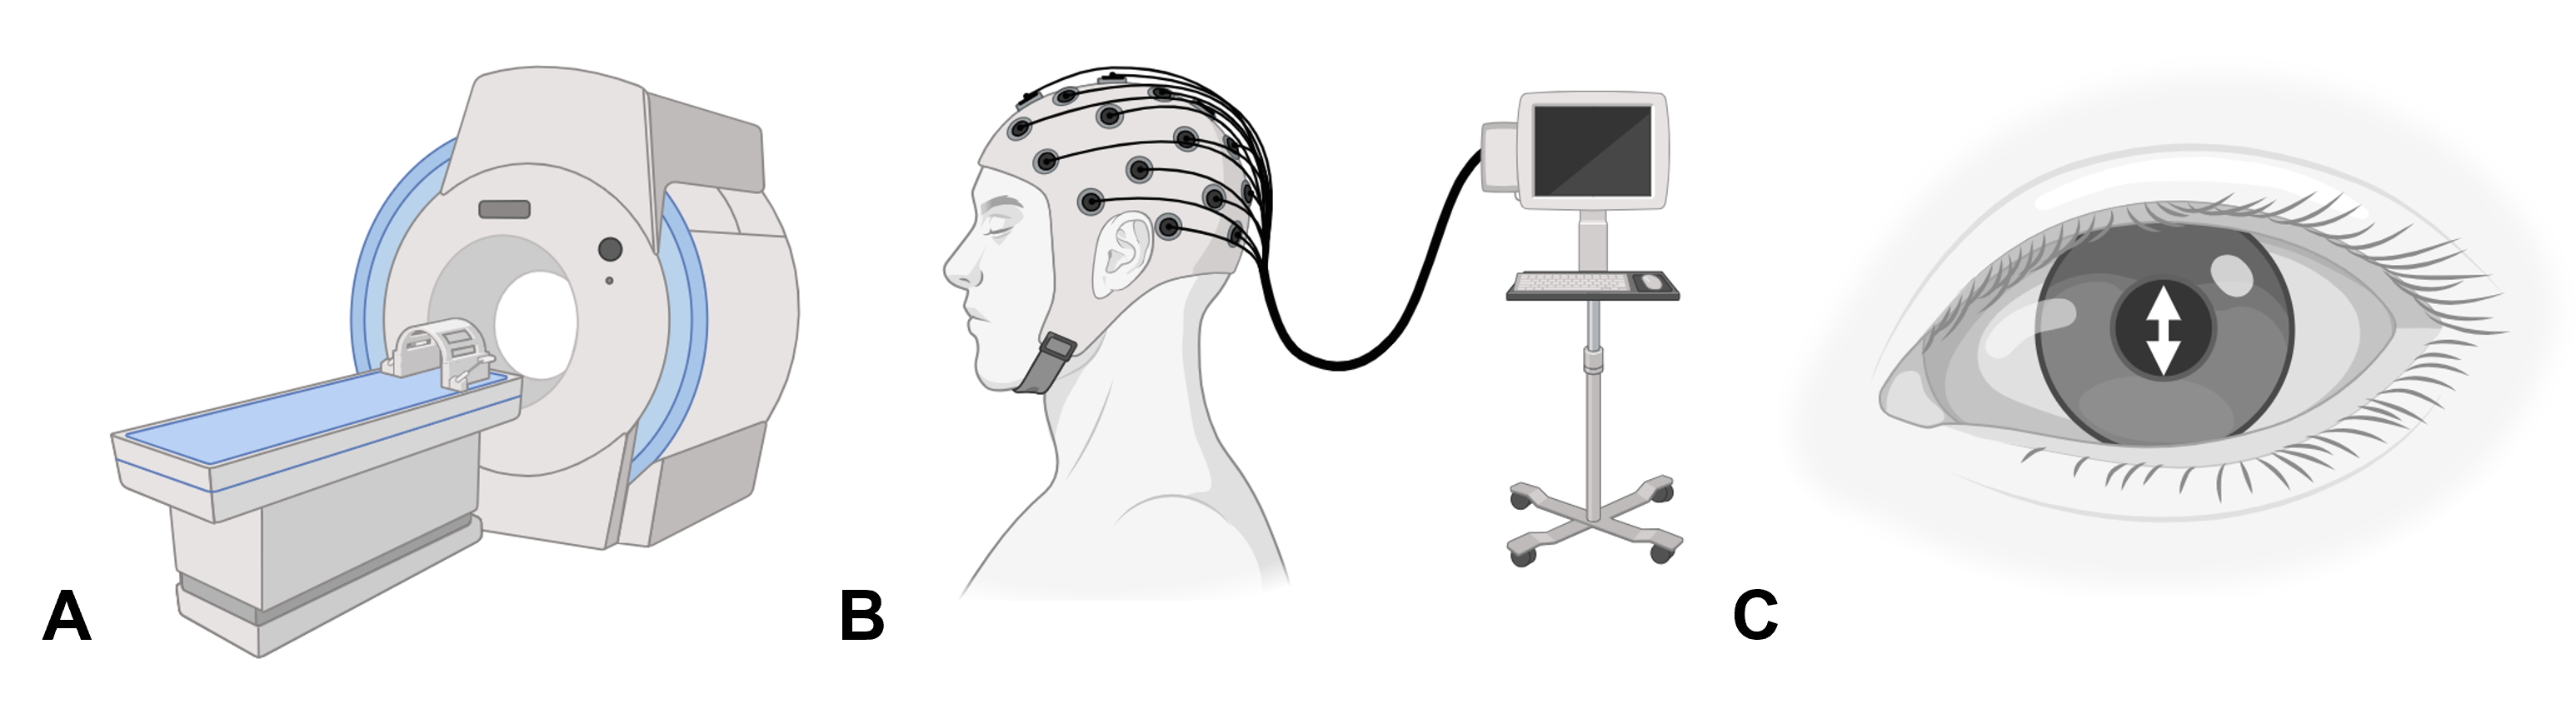
\includegraphics[width=1\textwidth, clip=true]{./Chapters/01_Introduction/Images/Methods}
	\caption{Methods to measure cognitive processing used in this thesis. (a) functional MRI (fMRI), (b) electroencephalography (EEG), and (c) pupillometry}
	\vspace*{-10pt}
	\label{fig:methods}
\end{figure}

An additional method of capturing cognitive resource allocation is to measure the pupil size during an event, known as pupillometry. This pupillary response is reliably shown to increase during events that require increased cognitive load, such as working memory demands or understanding complex sentences \citep{beatty1982}. The task-invoked pupillary response does not have an informative spatial dimension and therefore cannot inform us about other aspects of cognitive networks beyond attention. Yet, pupil dilations peak approximately one second after the occurrence of an event. This allows for a temporal precision in between those of fMRI and EEG, and provides valuable insight into processing load of a stimulus within an accessible, easy experimental set-up. 

\subsection{Neural infrastructure supporting language processing} 

With these and other neuroimaging methods, researchers have gathered evidence that the diversity of the necessary operations for communication is reflected in the brain regions and systems that support them. An initial necessary component is a memory system that has stored representations of concepts and the words that describe these concepts, located in the medial temporal lobe, middle temporal gyrus, and inferior temporal sulcus (MTG, pITS; see Fig~\ref{fig:methods}). To then concatenate these words into a sentence when speaking, or to dissect a sentence into parts and grasp their meaning, a system is needed that governs the relationship between words and can encode and decode these relationships from or into a specific structure, such as a word order. For example, it takes a certain mechanism to distinguish the different interpretations of the sentence `I saw the man with the binoculars'. A key role in this structure-building process is proposed for the left inferior frontal gyrus (LIFG) and the left MTG \citep{giglio2022,hagoort2017}. Then, as a last step, when formulating a message, articulatory movements must be prepared and executed, which is supported by the posterior part of the IFG and the premotor cortex \citep[PM; ][]{hickok2007}. On the comprehension side, upon hearing such a message, information flows from the auditory cortex, to the posterior superior temporal sulcus, to the frontal cortex \citep{friederici2012}. Of note is that most of these computations happen in the left hemisphere, especially in detecting and articulating speech. A critical role for language processing in the right hemisphere is reserved for understanding prosody, such as stress and intonation, and integrating an utterance in its context \citep{beaucousin2006,vigneau2011}.
\begin{figure}[!ht]
	\centering
	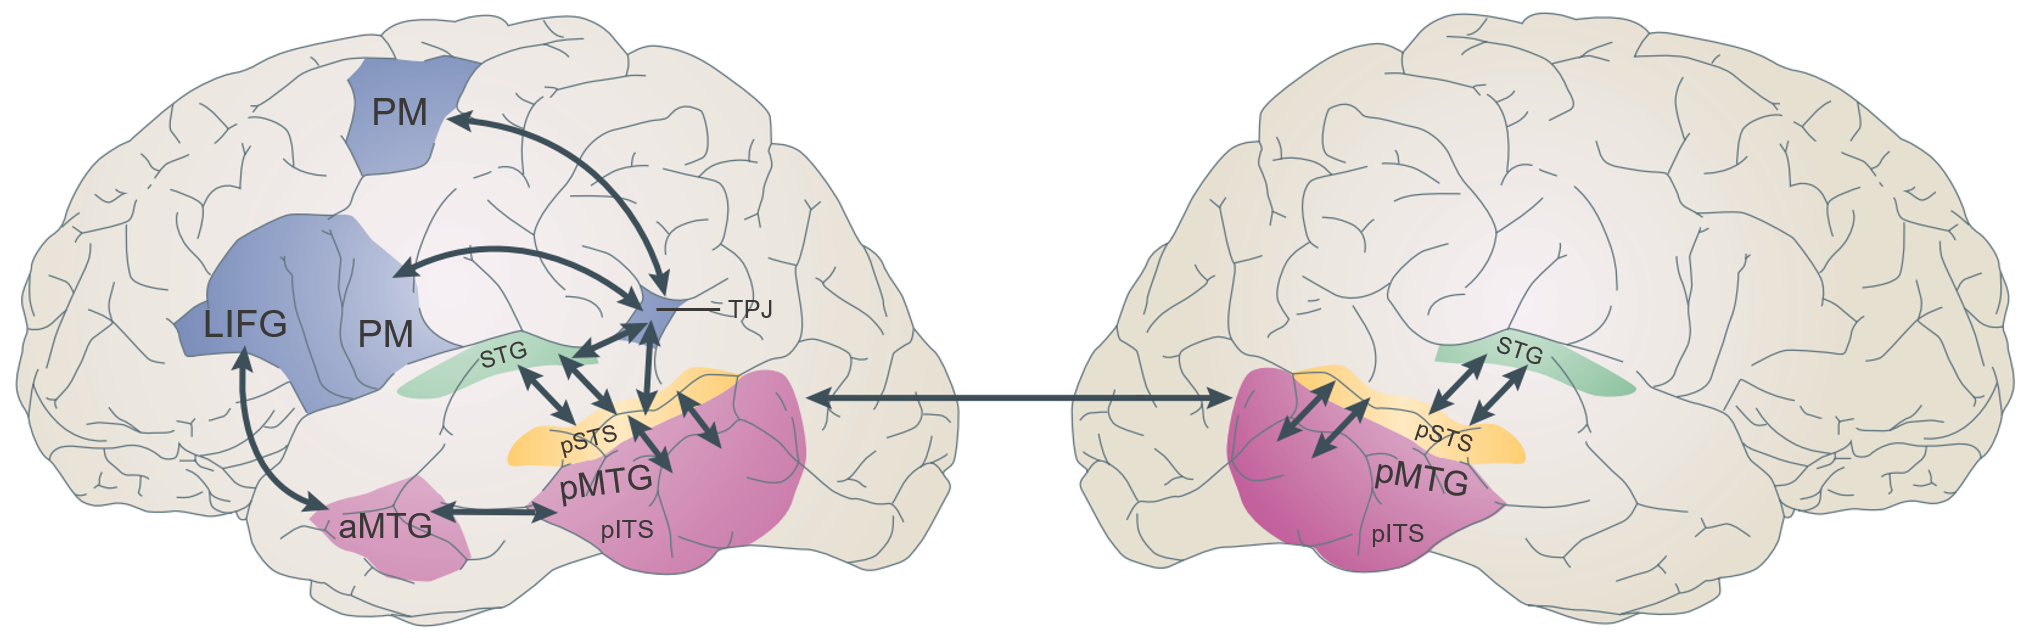
\includegraphics[width=.9\textwidth, clip=true]{./Chapters/01_Introduction/Images/Language_network_all_labels}
	\caption{Brain structures involved in language comprehension and production. Colors indicate different functional roles: pink = lexico-semantic interface, yellow = phonological network, green = spectrotemporal analysis of speech sounds, blue = articulatory network. LIFG = left inferior frontal gyrus, PM = premotor cortex, aMTG = anterior middle temporal gyrus, pMTG = posterior middle temporal gyrus, STG = superior temporal gyrus, TPJ = temporoparietal junction, pSTS = posterior superior temporal sulcus, pITS = posterior interior temporal sulcus. Figure adapted from \citet{hickok2007}}
    \vspace*{-10pt}
	\label{fig:language}
\end{figure}

Both speech recognition and production happen at fast rates: due to parallel activation of word candidates, word recognition takes around 200 milliseconds \citep{mcclelland1986}, whereas the trajectory of word production from conception to articulation can finish within 600 milliseconds \citep{indefrey2004}. These high speeds and accuracies are fundamentally subserved by white matter tracts connecting the aforementioned regions. Initial models of the language-related white matter connectome only included the arcuate fasciculus, the white matter bundle that connects frontal and posterior temporal brain regions. More recently, however, the involvement of white matter in relaying linguistic information across the whole brain has been called to attention \citep{przezdzik2019,tyler2007}.  

\subsection{Neural infrastructure supporting Mentalizing}

Several different types of task paradigms have been developed to test the neural mechanisms supporting mentalizing. Examples of these task types are tasks that elicit inferences of a falsely-held belief about a social situation \citep[False Belief task; ][]{baron-cohen1985}, comparisons of shapes that move in a socially or non-socially coded way \citep[Social Animations task; ][]{castelli2002}, or inferences of emotions from seeing a static image of eyes \citep[Reading the Mind in the Eyes task, or RMET; ][]{baron-cohen2001RMET}. The use of some of these different tasks leads to multiple problems for an accurate assessment of the ability to mentalize. First, it is unreasonable to believe that the different processes that underlie performance in these tasks probe the same psychological construct \citep{schaafsma2015}. Instead, what is more likely is that they share some but not all low-level processes that are operational during social interactions and observations, such as face recognition, self/other distinction, and tracking intentions. What further increases the variability of making inferences about mental states, is the fact that the content of the mental states being represented can very well be unique \citep{conway2019}. Consequently, neuroimaging studies have found that, depending on the type of mentalizing task used, a collection of different brain regions can be recruited, and is specific to the processes it taps into. Nevertheless, there is a set of core mentalizing brain regions, active in nearly all tasks claiming to test this construct, including the right temporoparietal junction (rTPJ) and medial prefrontal cortex \citep[mPFC; ][]{schurz2014}. 
\begin{figure}[!ht]
	\centering
	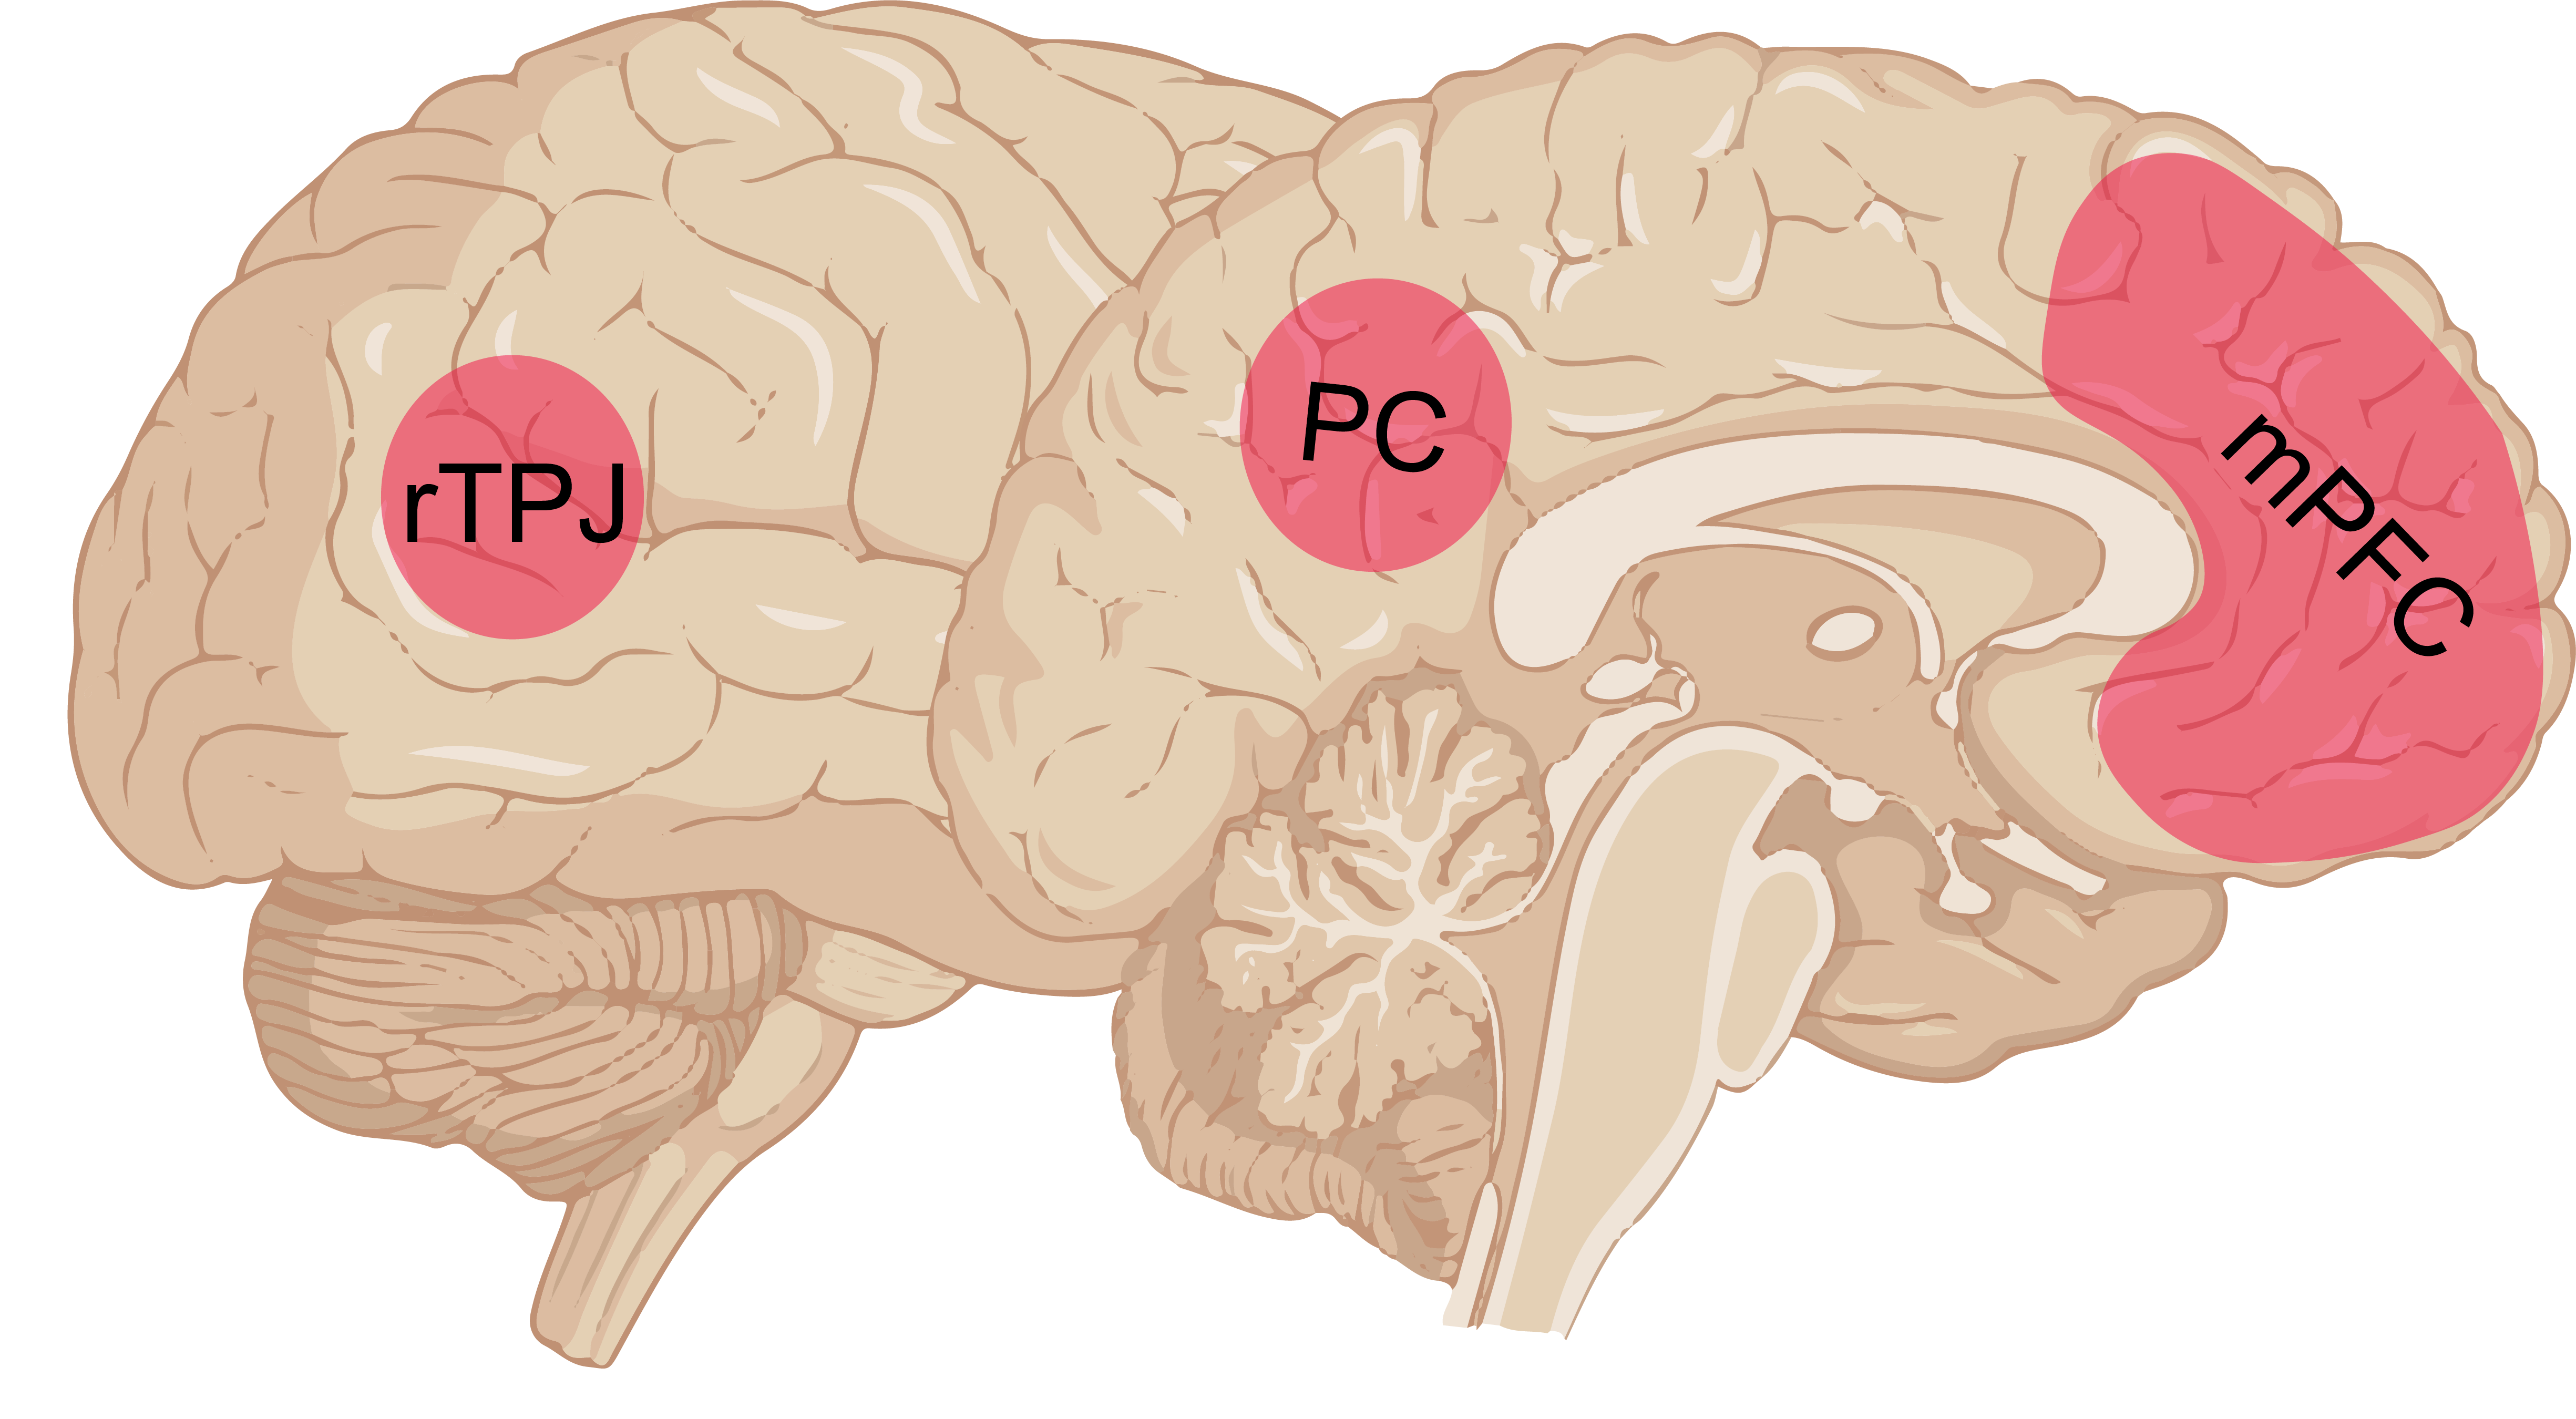
\includegraphics[width=.6\textwidth, clip=true]{./Chapters/01_Introduction/Images/Mentalizing_network}
	\caption{Brain structures involved in Mentalizing. mPFC = medial prefrontal cortex, PC = precuneus, rTPJ = right temporoparietal junction}
    \vspace*{-10pt}
	\label{fig:mentalizing}
\end{figure}

Another issue of these tasks is the lack of similarity to representing the minds of others in real-life communication. Many tasks require the participant to explicitly and verbally reason about a person’s belief, while in a dialogue this happens implicitly and spontaneously. An additional common feature of mentalizing tasks is that they do not feature dynamic stimuli of people or characters, but static pictures or drawings. It is of course difficult to single out and test specific low-level features related to mentalizing, while other features remain unchanged, and for the stimuli to retain naturalism, since mentalizing is very multi-faceted. Still, too few mentalizing studies have attempted to feature stimuli that resemble real-life communication \citep{gernsbacher2019,conway2019}.

The timing and automaticity of mental state inferences remain a contested issue. Some researchers propose a one-stage account, where both the speaker and partner's perspective are taken into account as early as possible \citep{brennan2009}. Others support a two-stage account, where the speaker's own perspective is processed first, and the partner's perspective is considered only when the speaker's perspective does not suffice for accurate and clear understanding \citep{barr2002}. However automatic perspective taking may be, encoding and decoding intentions of a partner happens very early in communication as shown by evidence from EEG experiments. In single-word scenarios, intentions seem to be integrated in word processing only 100 milliseconds after hearing the word embedded in a request or statement \citep{tomasello2022}. When uttering a request or statement, neural structures have integrated this communicative act as early as 600 milliseconds before starting to speak. Therefore, the necessity of predicting one's partner's intentions is reflected in its neural signatures.

\section{What happens when communication fails?}

As previously highlighted, successful communication requires many abilities and cognitive mechanisms to function interactively. Several (clinical) conditions exist in which one or more of these abilities are impaired, leading to a substantial impact on the quality of communication, social relationships and daily life in general. In this thesis, two of those conditions will be discussed: autism spectrum conditions and social anxiety.  

\subsection{Autism}

Autism spectrum conditions (hereafter: autism) are characterized by restricted and repetitive behaviors, altered processing of sensory stimuli, and social and communicative difficulties \citep{apa2013}. These difficulties can lead to mental health issues, apparent from the elevated prevalence of anxiety and depression in autistic children and adults \citep{hollocks2019,lai2019,vasa2020}. Difficulties in social situations emerge in early life for autistic children. They show less attention to their name being called, look less in the direction someone is pointing, and look less towards faces than geometric shapes \citep{goldberg2005,osterling2002,pierce2011}. This behavior is often followed by a delay in language development compared to non-autistic children \citep{kim2014}. These developmental delays are followed by difficulties in understanding non-literal language, such as ironic statements \citep{wang2006,deliens2018}, humor \citep{ozonoff1996}, or metaphors \citep{rundblad2010}. Differences can also be observed in less coherent speech, difficulties staying on topic when telling a story, and less attention to relevant information in understanding a story \citep{diehl2006,volden2002,yingsng2018}. In general, research shows that autistic individuals show decreased understanding compared to non-autistic individuals when the meaning of an utterance is dependent on the context \citep{angeleri2016,happe1997,loukusa2007,wadge2019}. 

Several theories have been proposed as an explanation for these behaviors. A decreased motivation to engage in social interactions is one of these theories \citep{chevallier2012}, yet it may be the case that social motivation is present to the same extent but expressed in a different manner \citep{escalona2002}. Improved local processing and decreased global processing in autism (known as weak central coherence) have been considered to underlie an increased propensity to interpret the literal meaning over the non-literal meaning of utterances \citep{happe1997}. This theory effectively distinguishes autistic from non-autistic individuals, but might poorly explain behavior on an individual level \citep{pellicano2006} and might not translate as a psychological construct in non-autistic individuals \citep{pellicano2005}. 

Perhaps the most widely held psychological theory underlying social behavior in autism is the viewpoint that they have a decreased mentalizing ability \citep{baron-cohen1985}. Recent evidence contesting this theory, however, is accumulating \citep{gernsbacher2019}, partly due to the drawbacks in mentalizing tasks mentioned earlier. More specifically, impaired mentalizing has been reported for other developmental conditions, rendering it not specific to autism \citep{jenkins1996,loukusa2014}. Impaired mentalizing also does not seem to be present in all autistic individuals, making it not a universal trait of autism \citep{happe1993,moessnang2020}. Lastly, several studies that show mentalizing differences do not control for language ability or use tasks that heavily rely on language \citep{gernsbacher2005}. This proves problematic given that the correlations between language ability and task performance are high \citep{capage2001,shaked2006}, and that structural language impairments occur in a substantial group of autistic individuals \citep{velikonja2019}. For these reasons, the claim that decreased mentalizing underlies social difficulties in autism has found itself on increasingly shaky ground. 

\subsection{Social Anxiety}

Social anxiety is characterized by an acute fear of being negatively evaluated in social situations. These situations include cases where feedback is expected such as giving a presentation or a job interview, but also cases where feedback is not likely such as during conversations or eating or calling on the phone in public \citep{apa2013}. This fear can be persistent enough for socially anxious people to avoid social situations altogether, leading to isolation, loneliness and in extreme cases substance abuse \citep{lemyre2019,lim2016}. A social anxiety disorder diagnosis can be designated when the fear and avoidance significantly affects functioning in daily life, although social anxiety can also be considered as a dimensional trait in non-clinical populations \citep{ruscio2010}. Known risk factors for social anxiety include genetic predisposition \citep{kendler1999}, cultural factors \citep{leung1994}, traumatic social experiences \citep{rapee2004}, and overprotective parents \citep{dulger2024,taylor2006}. Yet, a precise characterization of how these factors lead to the fear in social situations has not yet been identified. 

In addition to fear and avoidance of social situations, socially anxious individuals also experience difficulties during communicative situations. For one, they are anxious about how anxious they appear through signs as blushing, fidgeting or laughing nervously, and they in fact display these behaviors more often than non-socially anxious individuals \citep{voncken2008JAD}. Secondly, they are seen as less likable in general during conversation \citep{alden1995,creed1998,meleshko1993,voncken2008BJCP}. This may be a downstream consequence of other impaired aspects of interpersonal behavior in social anxiety, such as a lack of showing interest, responding, coherence, and silences \citep{voncken2008JAD}. Interestingly, this impaired social performance is only evident in conversational settings, not in one-way communication, such as when giving a speech, even though social anxious individuals rate their own performance as equally bad in both settings \citep{voncken2008JAD}. These negative self-beliefs about socially anxious individuals’ social competence and likeability are what is suggested to drive this impairment in social performance \citep{voncken2010}.

\section{What are the cognitive and neural mechanisms that underlie these forms of arduous communication?}

\subsection{Neural mechanisms underlying autism}

In search of a biomarker for autism, the anatomy and connectivity of the brain of autistic individuals has been studied intensively \citep[for a review]{pretzsch2022}. Large-sample datasets have pointed to differences in gray matter variations in frontal and subcortical areas, as well as functional connectivity in right fusiform gyrus compared to neurotypical brains \citep{mei2020,oblong2023}. Yet, many findings on atypical brain organization in autism fail to replicate between datasets or in matched samples \citep{he2020,koldewyn2014,mei2024,riddle2017}. 

Given the language impairment present in autism from early childhood into adulthood \citep{velikonja2019}, several studies have explored whether this impairment is related to differences in underlying brain activation. Existing studies indicate preliminary evidence for reduced activation in bilateral superior temporal gyrus to language and auditory stimuli and decreased cerebellum and right precentral gyrus activation \citep[for reviews]{groen2008,philip2012}. These findings, however, warrant the caveat that, first, some results are contested and do not replicate \citep{tryfon2018}, and second, that these studies include small sample sizes, often not exceeding more than 20 participants per group.

Despite these caveats, an atypicality in the autistic brain that is more consistently observed is the reduced left-lateralization of language functions. The pattern that language capacities are predominantly present in the left hemisphere \citep{broca1865,szaflarski2006} seems different for autistic participants, whose right hemisphere would be much more involved in linguistic processing \citep{eyler2012,jouravlev2020,knaus2008,knaus2010}. Furthermore, this reduced left-lateralization seems to be associated with impaired language performance \citep{cermak2022,lindell2013}.

In line with other neurolinguistic research, electrophysiological methods have been missing from studies on language and the brain in autism. As a result, information on the timing of linguistic processes is lacking. This is evident for research on both the general neural mechanisms underlying language processing and their lateralization. Lexical selection through oscillations \citep{bloy2019}, and speech detection through ERPs \citep{kasai2005,oramcardy2005} have been studied before, for which autistic and neurotypical participants have shown similar brain responses as of yet. Employing electrophysiology more widely to study the temporal aspects of language processing in the brain will be crucial to build informative cognitive models of language use in autism. 

Regarding research on mentalizing, few studies have investigated the neural mechanisms underlying this ability in autism, despite the pervasiveness of the reduced-mentalizing account. In two studies using False Belief tasks, lower activation was found in the rTPJ of autistic individuals than neurotypical individuals \citep{nijhof2018,yuk2018}. In addition, answering questions and reading passages about the intentions of others specifically elicited activation in the rTPJ for neurotypicals, but the mentalizing specificity of this area was decreased for autistic individuals \citep{lombardo2011,mason2008}. Most of these paradigms required linguistic processing and prompted explicit responses from the participant. A large-scale study that did not include these aspects, used a Social Animations task and interestingly did not find any regions that showed differences in brain activation in the two groups \citep{moessnang2020}. In sum, it seems that the rTPJ may harbor mentalizing processes specific to individuals without autism, depending on the type of task used.

\subsection{Neural mechanisms underlying social anxiety}

In the case of social anxiety, the neuroimaging literature points to higher activation of the fear network, comprised of the amygdala and anterior insula, in response to negative or threatening emotional stimuli \citep{bruhl2014,etkin2007}. The same meta-analysis also showed higher activation in medial and lateral prefrontal regions, suggested to reflect altered top-down control \citep{bruhl2014}. Conversely, Koban and colleagues (\citeyear{koban2023}) found a diminished recruitment of a frontoparietal network in socially anxious participants. This brain network was shown to support a positive bias of self-evaluation updating in control participants. These findings are contradicting, particularly on activation in the dorsolateral prefrontal cortex, but this might be explained by the different tasks used in these studies (observing faces vs. receiving negative feedback about oneself). Nevertheless, this diminished positive updating bias in social anxiety identified by Koban and colleagues (\citeyear{koban2023}) could lead to the bias for negative social cues that is apparent in their behavior \citep{alvi2020}.

A glaring omission from studies on social anxiety, either including or excluding neuroimaging methods, is one previously mentioned in the context of mentalizing tasks, which is a lack of naturalistic and non-evaluative paradigms assessing higher-level social cognition \citep{freitas-ferrari2010}. In the past decade, a decreased mentalizing ability has been suggested to underlie fear in social situations in socially anxious individuals \citep{hezel2014}. However, the most commonly used task, the RMET, operationalizes reading mental states as looking at a pair of eyes \citep[for a review]{baez2023}. Moreover, the only neuroimaging study claiming to test mentalizing in social anxiety comprised of a task in which participants had to make economic decisions by considering the mental state of their partner, shown as a static image of a face, or a computer \citep{sripada2009}. In addition to the fact that these tasks do not resemble real-life situations, they explicitly prompt the participants to perform on a task. This evaluative setting may increase performance anxiety in the socially anxious individuals. In sum, performing naturalistic and non-evaluative studies on social cognition is necessary to provide a comprehensive and complete picture of social anxiety. This is especially important given the impaired abilities of socially anxious individuals in interpersonal behavior and their tendency to direct their internal focus on themselves instead of the ongoing conversation.


\section{Objectives and outline}

The objectives of this thesis were twofold: first, to uncover the neurocognitive mechanisms underlying mental state inferencing and observing social interactions in autism and social anxiety, and second, to investigate the neurocognitive features of linguistic structure building and lateralization in autism. 

The outline of the thesis is as follows: in chapter~\ref{ch:mentalizing_asc}, the aim was to assess the cognitive functioning of neurotypical and autistic participants during a naturalistic movie in order to investigate differences in mental state inferencing and navigating unpredictable contexts. To that end, we showed them a short nonverbal Pixar film involving social interactions while recording their brain and pupil responses in an MRI scanner. Together with a post-scanning inquiry about the plot of the movie, we studied the propensity for mentalizing by contrasting events with and without scenes that prompted mental state inferences. Additionally, we compared the variability of brain and pupil responses within the groups of autistic and neurotypical individuals to assess the idiosyncrasy of each group during the observation of interactions. In chapter~\ref{ch:mentalizing_sa}, the goal was to determine whether an aberrant way of mental state inferencing was related to social anxiety during observations of social interactions. For that reason, we measured brain and pupil responses to the same short movie as in chapter 2 but for socially anxious and matched control individuals. Activation specific to mental state inferencing and variability of neural response were again measured with fMRI and pupillometry and compared between groups. Furthermore, the participants' heart rate was measured and their verbal reasoning about the emotions of characters was gauged, in line with the goal to assess propensity for inferencing about emotions and mental states and relate it to anxiety during the non-evaluative movie-watching task. In chapter~\ref{ch:language_asc}, we addressed the question whether linguistic structure building induced different neural mechanisms in neurotypical and autistic participants. This was done by measuring the neural oscillations with EEG in autistic and neurotypical individuals who read sentences or non-word lists. The timing and the extent of lateralization of these linguistic processes was assessed and compared for the two groups. In chapter~\ref{ch:discussion}, I summarize and integrate the findings from these chapters in a general discussion, in addition to an outlook on future research.
